\chapter{Case study}

\begin{chapterintro}
In this chapter we are going to describe two selected use cases that represents how the gamer will interact with the application.
Firstly, we will describe the gamer interaction with the playing instrument game mode. Secondly, we will study the conduct orchestra game mode 
\end{chapterintro}

\cleardoublepage

\section{Introduction}

In both use cases, two actors are involved, the gamer and the instrument recognition algorithm.

\begin{table}[!htpb]
\centering
\begin{tabular}{|c|c|x{6cm}|}
\noalign{\hrule height 2pt}
\textbf{Actor identifier} & \textbf{Role} & \textbf{Description}\tn
\hline
ACT-1 & Gamer & End user that plays the game using the physical instruments and the application\tn
\hline
ACT-2 & {Instrument recognition algorithm} & Algorithm that detects what physical figure has been placed on the application recognition zones\tn
\noalign{\hrule height 2pt}
\end{tabular}
\caption{Actors list}
\label{tab:actoresusecase}
\end{table}

In the following sections we will explain two of the principal application game modes:

\begin{itemize}
\item \textit{Playing instrument game mode} detailed in section \ref{sec:playinginstrumentgm}.
\item \textit{Conducting orchestra game mode} detailed in section \ref{sec:conductingorchestragm}.
\end{itemize}

The \textit{Gamer} is able to access to both game modes from the application home screen, using one of the physical instrument miniature. Within each game mode, the gamer is able to interact with every component in order to select other musical instrument, change melodies, play an instrument, watch a play instrument demo, choose what instruments must be playing, etc.

The \textit{Instrument recognition algorithm} allows the application engine to detect which physical instrument miniature has been placed on the screen recognition zones. As a result, the gamer is able to interact with the game mode using the physical instrument miniatures.

\newpage
\section{Playing instrument game mode}
\label{sec:playinginstrumentgm}

In this section we are going to detail the whole application flow within the \textit{Playing instrument game mode}. This game mode is defined in the application workflow represented in figure \ref{subsec:playinstrument_arch}.

Firstly, the \textit{Gamer} has to open the application that have been previously installed on their device from either \textit{Android Play Store} or \textit{iOs App Store}. Also, the gamer must have purchased the physical instrument miniatures. These miniatures are necessary to interact with the application so that we can access to different game modes and change instruments inside them.

After opening the application the home screen is loaded. We can see game home screen in Figure \ref{fig:home_screen}.

\begin{figure}[ht!]
	\centering
	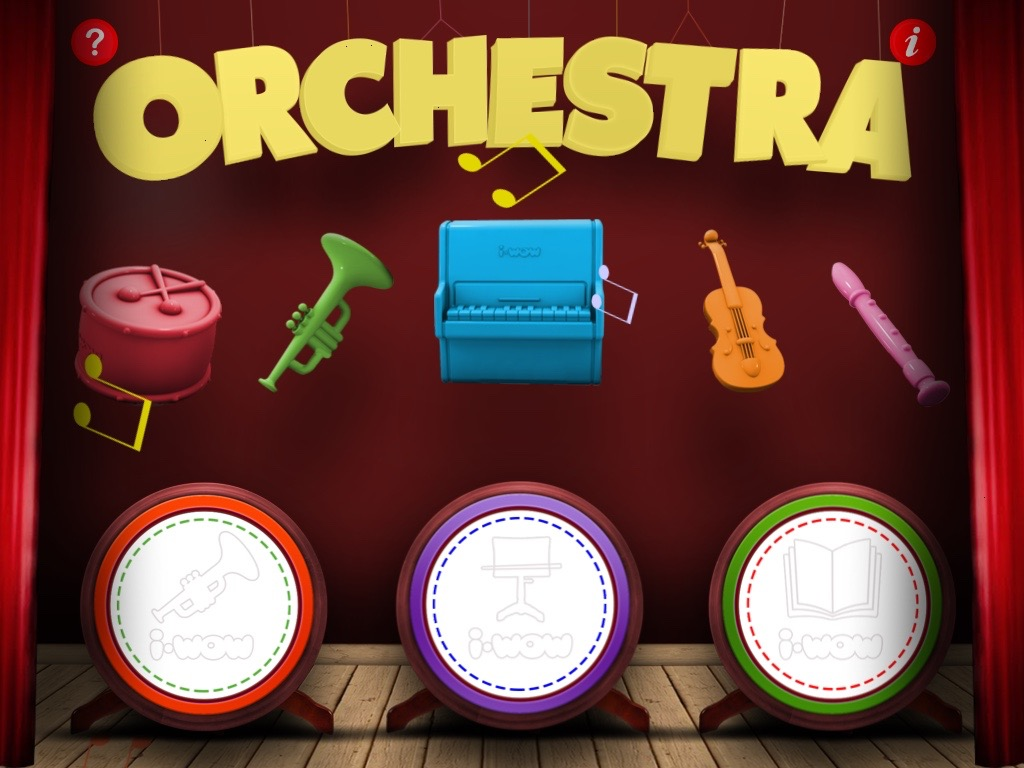
\includegraphics[width=400pt]{graphics/use-case/home_screen.jpg}
	\caption{Application Home Screen}
	\label{fig:home_screen}
\end{figure}

\newpage

By interacting with this home screen we have the possibility to access to each of the three game modes availables. In case it is our first contact with the game and we do not know how to interact with it, we can get some help touching the help button (represented with a question mark at the top left corner of the home screen). The help for the home screen is shown in Figure \ref{fig:help_home_screen}.

\begin{figure}[ht!]
	\centering
	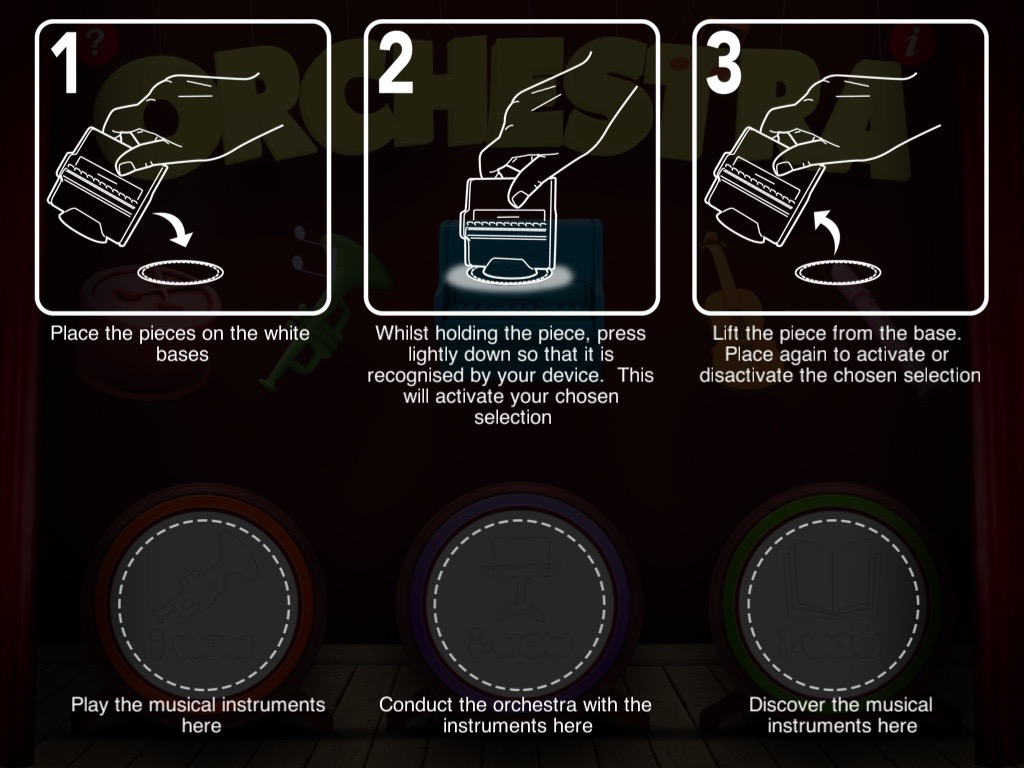
\includegraphics[width=400pt]{graphics/use-case/help_home_screen.jpg}
	\caption{Help Home Screen}
	\label{fig:help_home_screen}
\end{figure}

As we can see in Figure \ref{fig:help_home_screen}, in order to access to one of the three game modes, we should place one of the physical instrument miniature (from now on piece) on one of the instrument recognition zones (from now on white bases). After placing it, we just have to hold and press lightly down the piece so that the application can recognize it. This recognition is processed within the \textit{Instrument recognition algorithm}. After it, we can lift the piece from the white base and place another one if we can access to another game mode if we get back the home screen.

In this case, we want to access to the \textit{Playing instrument game mode}, so we choose one of the pieces and place it on the left white base so that we can access to the play instrument game mode. In our case, we have chosen the percussion piece. After situating the percussion piece on the left white base, a new screen, showed in Figure \ref{fig:playing_xylo_start_screen}, is opened.

\begin{figure}[ht!]
	\centering
	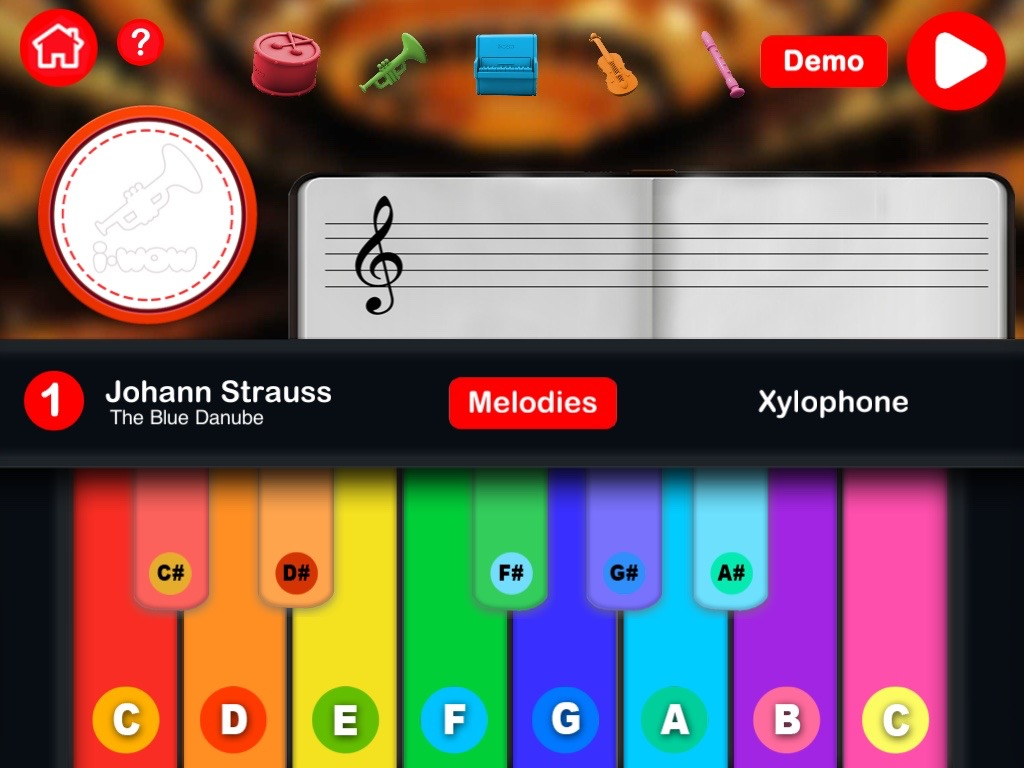
\includegraphics[width=400pt]{graphics/use-case/playing_xylo_start_screen.jpg}
	\caption{Xylophone playing instrument game mode}
	\label{fig:playing_xylo_start_screen}
\end{figure}

\FloatBarrier

\newpage
\section{Conducting orchestra game mode}
\label{sec:conductingorchestragm}

Conducting orchestra game mode

\newpage
\section{Conclusions}

